\subsection{Criteri di Valutazione}\label{ssec: Criteria}

I criteri per la valutazione e il confronto dei diversi algoritmi soono stati : 
\begin{itemize}\label{eq: confusion matrix}
    \item Accuracy: \begin{equation}
        Accuracy= \frac{TP+TN}{TP+TN+FP+FN}
    \end{equation}
    \item Precision: \begin{equation}
        Precision= \frac{TN}{TN+FP}
    \end{equation}
    \item Recall: \begin{equation}
        Recall= \frac{TP}{TP+FN}
    \end{equation}
    \item F1-score: \begin{equation}
        F1-score= \frac{2 *  Precision * Recall}{Precision + Recall}
    \end{equation}
    
\end{itemize}
Dove TP sono i \textit{True Positive}, TN sono i \textit{True Negative}, FP sono i \textit{False Positive} e i FN sono i \textit{False Negative}. 
\newline Avendo delle classi bilanciate nel daset, come mostrato nella fig. \ref{fig:target}, ho tenuto in considerazione l'accuracy come metrica di confronto più indicativa tra le prestazioni dei modelli. Da qui la scelta nella cross validation e nell'ensamble di usare come parametro "scoring" l'accuracy. Quest'ultima fornisce un'idea di quanti sample predetti sono effettivamente della classe giusta. L'accuracy "totale" sarebbe totalmente inappropriata nel caso di dataset sbilanciati, per i quali dev'essere valutata l'accuracy per \textbf{ogni} classe. Potrebbe infatti dare risultati fuorvianti, poichè avendo molte istanze della stessa classe, si avrebbe una accuracy molto alta proprio perchè l'algoritmo riesce a prevedere molto bene la classe che ha "visto" più volte, ma non riesce a discernere una classe da un'altra. In caso di sbilanciamento del dataset si tende a preferire l'F1-Score poichè, essendo una media armonica che unisce Precision e Recall in un unica metrica, attribuisce un peso maggiore ai valori piccoli. Quindi usare F1-Score è utile sopratutto nei casi in cui per una o più classi ci sono pochi positivi, come nei dataset sbilanciati. 
\newline I quattro valori \textsc{TP,TN, FP, FN} si possono visualizzare graficamente attraverso quella che viene definita come \emph{Confusion matrix}.

\begin{figure}[H]
    \centering
    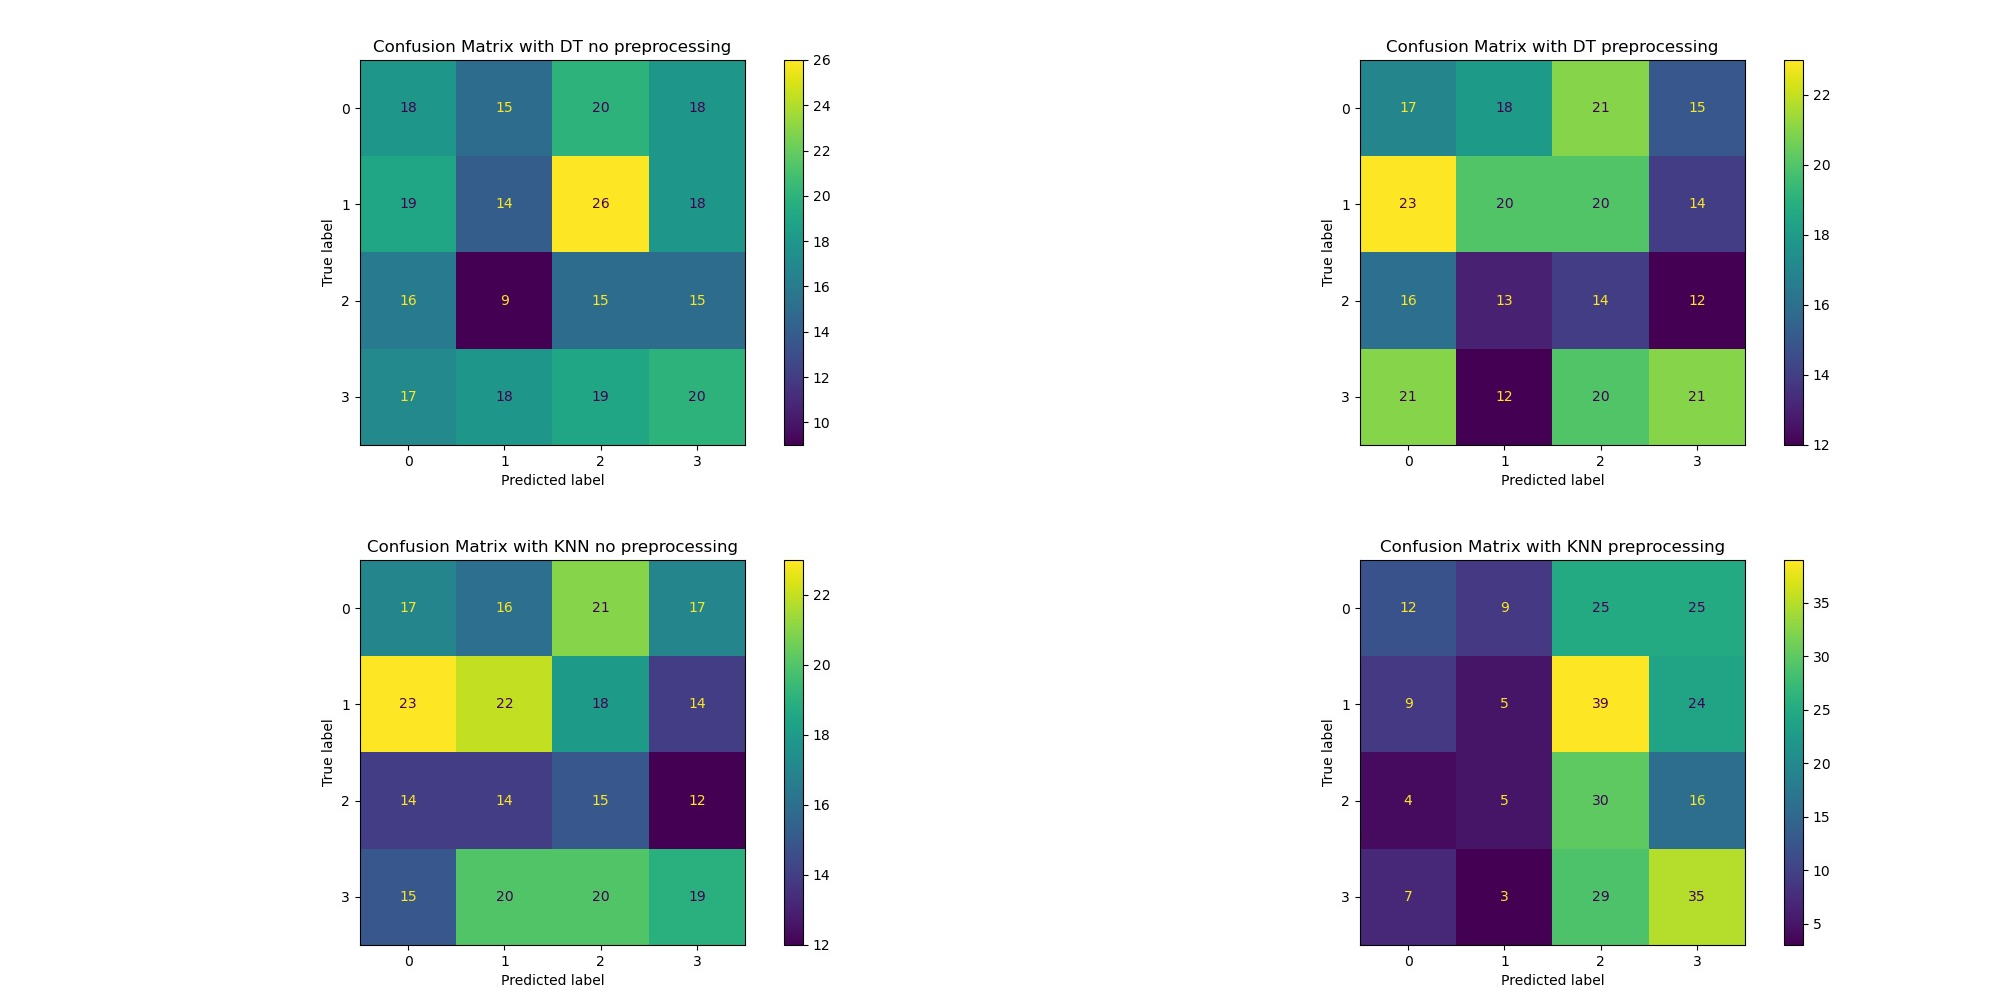
\includegraphics[width=1.1\columnwidth]{figures/Merge of Confusion Matrix.png}
    \caption{Le 4 confusion Matrix}
    \label{fig:target}
\end{figure}

Un'altra metrica importante da considerare è la ROC curve, ovvero la Relative Operating Characteristic. Infatti variando la soglia di classificazione si ottengono valori diversi per le metriche sopra menzionate. Per cambiamento della soglia di classificazione si intende la modifica dei paramentri del classificatore. 
La curva ROC viene creata tracciando il valore del True Positive Rate (TPR, frazione di veri positivi) rispetto al False Positive Rate (FPR, frazione di falsi positivi) a varie impostazioni di soglia. La curva ROC è quindi il tasso dei veri positivi in funzione del tasso dei falsi positivi.
\newline Per ultima abbiamo la curva Precision versus recall. Ricordo che la Precision o Specificity è la probabilità che un falso positivo ritornato dal classificatore sia corretto mentre la Recall è la percentuale di positivi riconosciuti correttamente. 
